% title: A memoized primitive call can reuse a cached result
% description: Within a memoize context, an eligible primitive call looks up its primitive identity, input values, and parameters. A hit reuses the result; a miss runs the primitive and stores its result.
\documentclass[tikz,border=5pt]{standalone}
\usetikzlibrary{arrows.meta,shapes.geometric}
\begin{document}
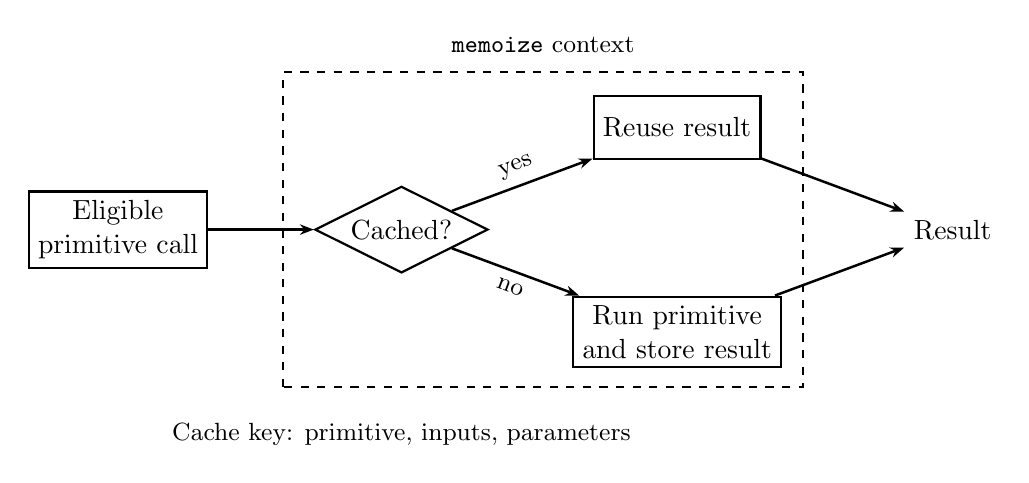
\begin{tikzpicture}[
    box/.style={draw, line width=0.8pt, minimum height=0.8cm,
                minimum width=1.8cm, align=center},
    flow/.style={-{Stealth[length=5pt]}, line width=0.9pt},
    note/.style={font=\small, align=center},
    choice/.style={diamond, draw, line width=0.8pt,
                   aspect=2, inner sep=2pt, align=center},
]

    \node[box] (call) at (0,0) {Eligible\\primitive call};
    \node[choice] (cache) at (3.6,0) {Cached?};
    \node[box] (reuse) at (7.1,1.3) {Reuse result};
    \node[box] (run) at (7.1,-1.3) {Run primitive\\and store result};
    \node (out) at (10.6,0) {Result};
    \draw[flow] (call) -- (cache);
    \draw[flow] (cache) -- node[above,sloped,note] {yes} (reuse);
    \draw[flow] (cache) -- node[below,sloped,note] {no} (run);
    \draw[flow] (reuse) -- (out);
    \draw[flow] (run) -- (out);
    \node[note] at (3.6,-2.6) {Cache key: primitive, inputs, parameters};
    \draw[dashed,line width=0.7pt] (2.1,-2) rectangle (8.7,2);
    \node[note] at (5.4,2.35) {\texttt{memoize} context};

\end{tikzpicture}
\end{document}
